
\begin{center}
\thispagestyle{empty}


\vspace{.5cm}

%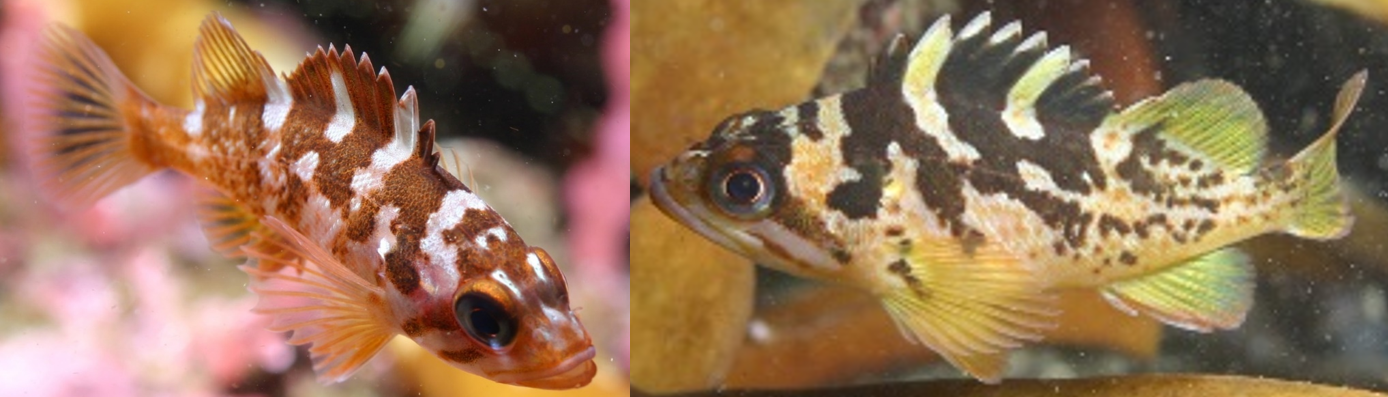
\includegraphics{cover_photo}~\\[1cm]
\pdftooltip{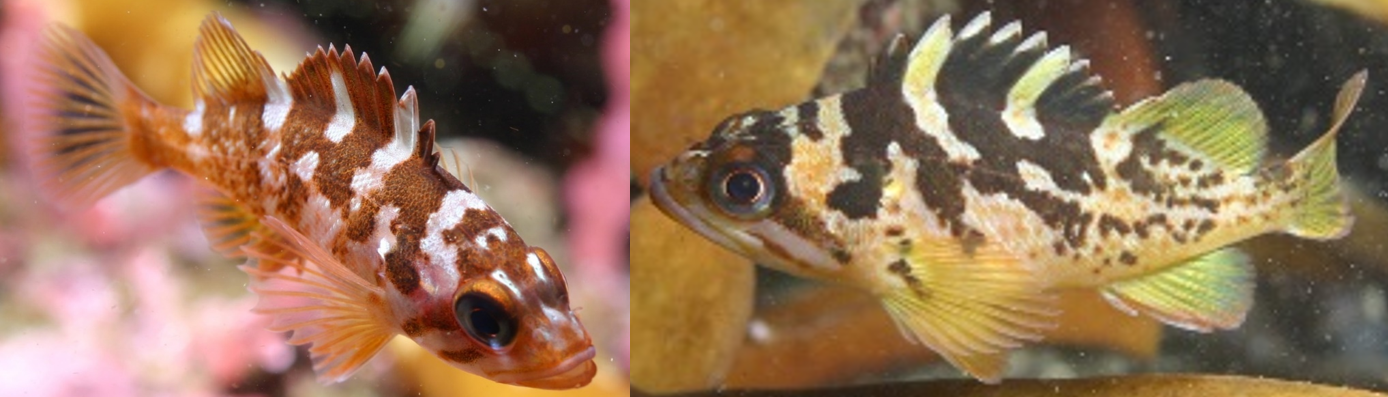
\includegraphics{cover_photo}}{This is a fish.}
Gopher rockfish (left) and black-and-yellow rockfish (right).      
\small
Photos by Steve Lonhart.

\vspace{.3cm}


Melissa H. Monk\textsuperscript{1}\\
Xi He\textsuperscript{1}\\

\vspace{.5cm}

\small
\textsuperscript{1}Southwest Fisheries Science Center, U.S. Department of Commerce, National Oceanic and Atmospheric Administration, National Marine Fisheries Service, 110 McAllister Way, Santa Cruz, California 95060\\

\vspace{1.5cm}


%\vfill
DRAFT SAFE\\
Disclaimer: This information is distributed solely for the purpose of pre-dissemination
peer review under applicable information quality guidelines. It has not been formally
disseminated by NOAA Fisheries. It does not represent and should not be construed to
represent any agency determination or policy. 

\vspace{.1cm}
%Bottom of the page
{\large \today}


\newpage{\thispagestyle{empty}}


\begin{flushleft}
This report may be cited as:

Monk, M. H.  and X. He. 2019. The Combined Status of Gopher (*Sebastes carnatus*) and Black-and-Yellow Rockfishes (*Sebastes chrysomelas*) in U.S. Waters Off California in 2019. Pacific Fishery Management Council, Portland, OR. Available from http://www.pcouncil.org/groundfish/stock-assessments/
\end{flushleft}

\maketitle

\pagenumbering{roman}
\setcounter{page}{1}
\end{center}


